% primary responsibility: CAS+Phil

\section{Design}

The goal of our system is two fold: block websites that are not part of the
white list and to record network statistics about the Internet usage of the
family. The second goal is important because it is not enough to just block
unwanted websites, health Internet usage habits must be developed as well. By
logging Internet usage, parents can identify any unhealthy behaviors with the
use of the Internet. For example, say a teenager is staying up late to use the
Internet and the website they are viewing is on the whitelist. The content the
teenager is viewing might not be bad (such as a simple Internet game), but
staying up late is not a healthy habit. With this information, the parents are
able to address this problem in a direct manner.

For both blocking and reporting, we used the intrusion detection system (IDS),
Snort~\cite{snort}. An IDS is a piece of software that sits on individual
clients (called host based IDS or HIDS) or on a network (called network based
IDS or NIDS). It monitors traffic that passes through it and detects if any
type of attack common is occurring. It records this information in a database
and notifies an network administrator if it detects any serious problems.

The IDS' host can be installed in either of two topological modes: in-line and
stub.
%
In-line installation requires the IDS host to forward every packet entering or
leaving the network.
%
It guarantees that the IDS will able to process (or block) every packet, at
the expense of slowing down network communication to the speed that the IDS
host can handle.
%
If the in-line IDS host becomes overloaded or fails, all network communication slows
or stops.
%
On the other hand, a stub-installed IDS host requires a network hub (\emph{not} a
switch).
%
(Recall that a network hub sends all traffic it receives out on all its ports,
unlike a switch, which determines each packet's destination host, and only
sends the packet out on the appropriate port. )
%
The hub allows the IDS on the IDS host to silently listen to all traffic
passing through the hub, and if it determines a TCP packet is problematic, the
hub allows the IDS to interrupt the packet's TCP connection by sending a TCP
reset signal to the packet's source and destination hosts.
%
If a stub-installed IDS becomes overloaded or fails, it allows some or all
packets through without logging and/or interrupting them.

While passing unfiltered packets admittedly weaken the primary goals of
KindSicher, we opted for a stub-configured IDS host, on the theory that it is
better to have weaker browsing protection than to risk children not being able
to communicate in an emergency (e.g. using an internet phone to call a parent
after a sibling trips and breaks an arm).



% \newcommand*\ifline[3]{%
        % \ifthenelse{\value{VerbboxLineNo} = #1}{#2}{#3}}

% \begin{verbbox}[\ifline{6}{\vspace{10pt}}{\ifline{10}{\vspace{3pt}}{\ifline{12}{\vspace{3pt}}{\ifline{14}{\vspace{10pt}}{}}}}]
\begin{verbbox}
<rule_action> <protocol>
    <src_ip_addr> <src_port>
    <direction>
    <dst_ip_addr> <dst_port>
    (<meta_data>)


<rule_action>: alert, log, pass, activate,
    dynamic, drop, reject, sdrop

<protocol>: tcp, udp, ip, etc.

<direction>: ->, <-, <>

Example:
reject tcp
    any any
    <>
    10.0.0.10 80
    (sid: 1; msg: "rejecting!";)

\end{verbbox}

\begin{figure}[!t]
    \centering
    \theverbbox
    \caption{The general syntax of a Snort rule with an example.}
    \label{fig:rule_syntax}
\end{figure}

Snort is rule based. This means that a user can write rules that if the rule
conditions are met, Snort performs an action. Figure~\ref{fig:rule_syntax}
shows the general syntax of a rule. There are communities of Snort users that
write rules for common attacks and network problems so that typical users do
not need a deep knowledge of intrusion detection to get benefit from Snort.

% TODO: Describe network topology
\begin{figure*}[!t]
    \centering
    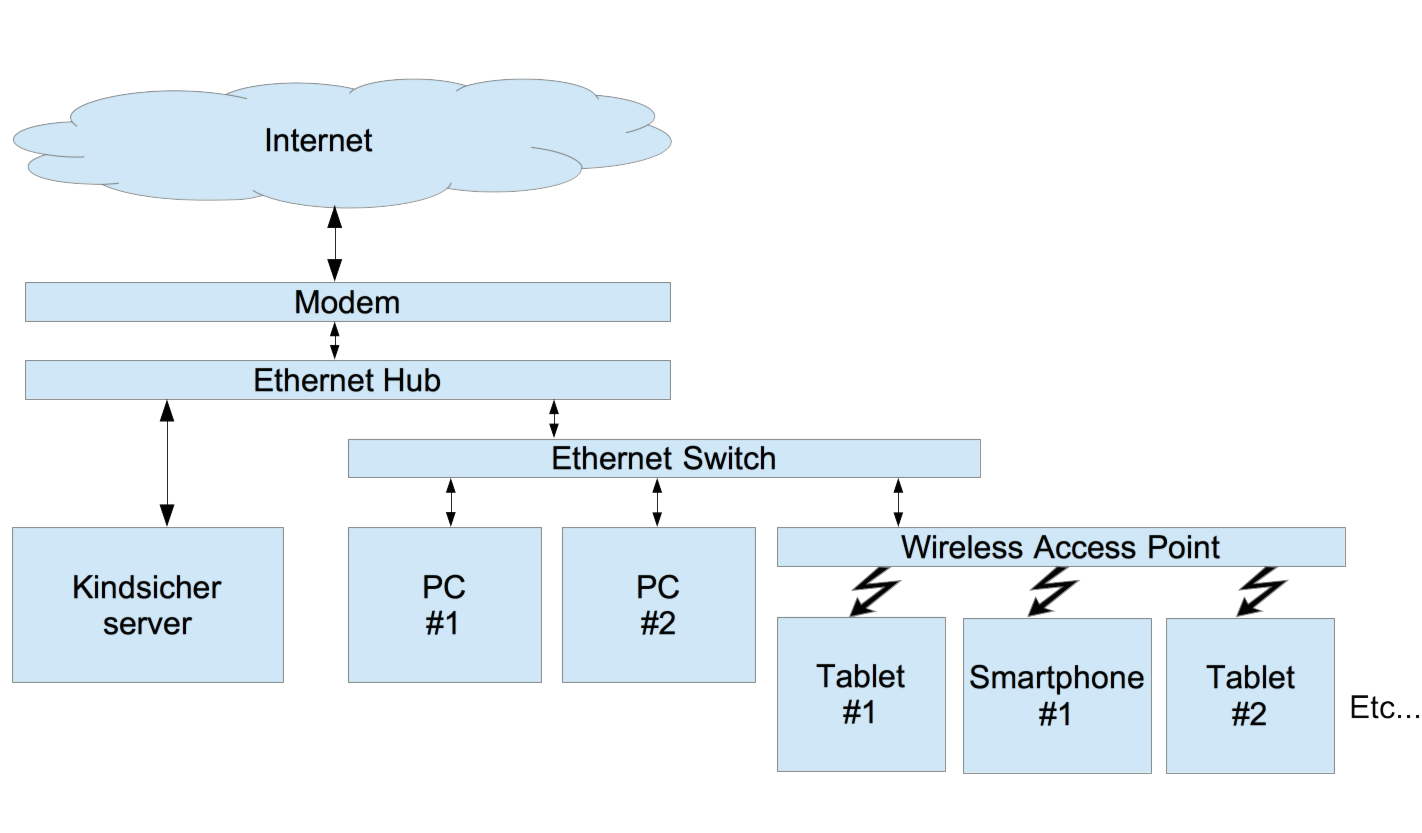
\includegraphics[width=2\columnwidth]{figures/topology}
    \caption{The network topology of the Kindsicher system. An Ethernet hub is
        used to broadcast all traffic from the Ethernet switch to the
        Kindsicher server. The Ethernet switch contains a mixture of PCs and
        wireless clients. Any device that connects to the Ethernet switch will
        be automatically protected by the Kindsicher server.}
    \label{fig:topology}
\end{figure*}

How Snort was used to accomplish each goal (blocking and reporting) is outlined
in the sections below.

% ==================================================
\subsection{Login}

The TCP/IP protocol, and the HTTP protocol that rides on top of it, identify
the sending computer, \emph{NOT} the user name on that computer.
%
Since Kindsicher's goal is to restrict access for children, not for adults,
the only way to distinguish between children's internet access and adults'
access is to designate certain computers for children's use only, and other
computers for adults' use only.
%
Thus, there needs to be some mechanism to ensure that the children can only
log into hosts designated for children.

The network we used for testing uses SNISR
%
\footnote{ SNISR is a network login and directory information system, akin to
LDAP, NIS, or Hesiod.  Its signature advantage is that all clients have a
local record of account and group information at all times, so mobile clients
can be disconnected from the network and reconnected at will.  For more
information, see http://www.mathoni.net/cas/swforge/snisr for more
information. }
%
for login directory services.
%
The current released version, SNISR 1.1, allows any user to log in on any host.
%
Part of this project, therefore, was upgrading SNISR to allow the network
administrator to specify classes of hosts that only certain users could log
into.
%
SNISR 2.0's baseline ALPHA\_6 contains this feature, and is expected to begin
beta testing soon.


